\chapter{Problemanalyse}
\label{chapter:problemanalyse}

\section{Databasedesign}
\label{section:databasedesign}

På baggrund af kravene til systemet beskrevet i forrige kapitel, ser vi behov for at implementere de tabeller i en relationsdatabase, som i de næste sektioner vil blive beskrevede.

Med hensyn til valg af relationsdatabase, ville et lokalt databasesystem være at foretrække, da reservationssystemet som nævnt ikke skal håndtere opdateringer over nettet eller køres på mere end een maskine ad gangen. Det endelige valg er derfor faldet på SQLite\footnote{\url{https://sqlite.org/}} frem for den af pensum gennemgåede MySQL\footnote{\url{http://www.mysql.com/}}.

\subsection{Film}

For at have en funktionel biograf, er det nødvendigt at have en film. 
Filmen/e får tildelt et navn.

\subsection{Sal}

Udover en film, er det også nødvendigt at have en sal for at vise filmen. På samme måde som \textit{Film}, får salene også tildelt navn. For at det ikke skal være alt for ubehageligt for publikum, så har salene også et antal rækker og sæder. 

\subsection{Forestilling}

En forestilling er en film, som bliver vist i en given sal på et givet tidspunkt.

\subsection{Reservation}

Det er muligt at reservere sæderne for at se en film. Dog kun, hvis der er en forestilling. Til reservationerne skal der oplyses et telefonnummer, og hvor mange billetter reservationen skal have.

\subsection{Billet}

Billetterne er en liste som tilhører \textit{Reservation}, hvor der er tildelt en række og et sæde pr. billet. 

\section{Præsentation af data}

Det første skridt mod et program er ofte et mockup. Et mockup visualiserer en idé, og får en brainstorm til at være mere konkret. Vi har valgt at bruge programmet Balsamiq Mockups.

Det står i problemformuleringen, at Bookie ikke skal være indviklet, hvilket bliver reducéret til, at Bookie kun skal kunne det mest basale, som et reservationssystem kræver. Data er en nødvendighed, men der er forskellige måder at repræsentere den på.

\begin{figure}[h]
  \centering
  \begin{minipage}[b]{0.44\linewidth}
  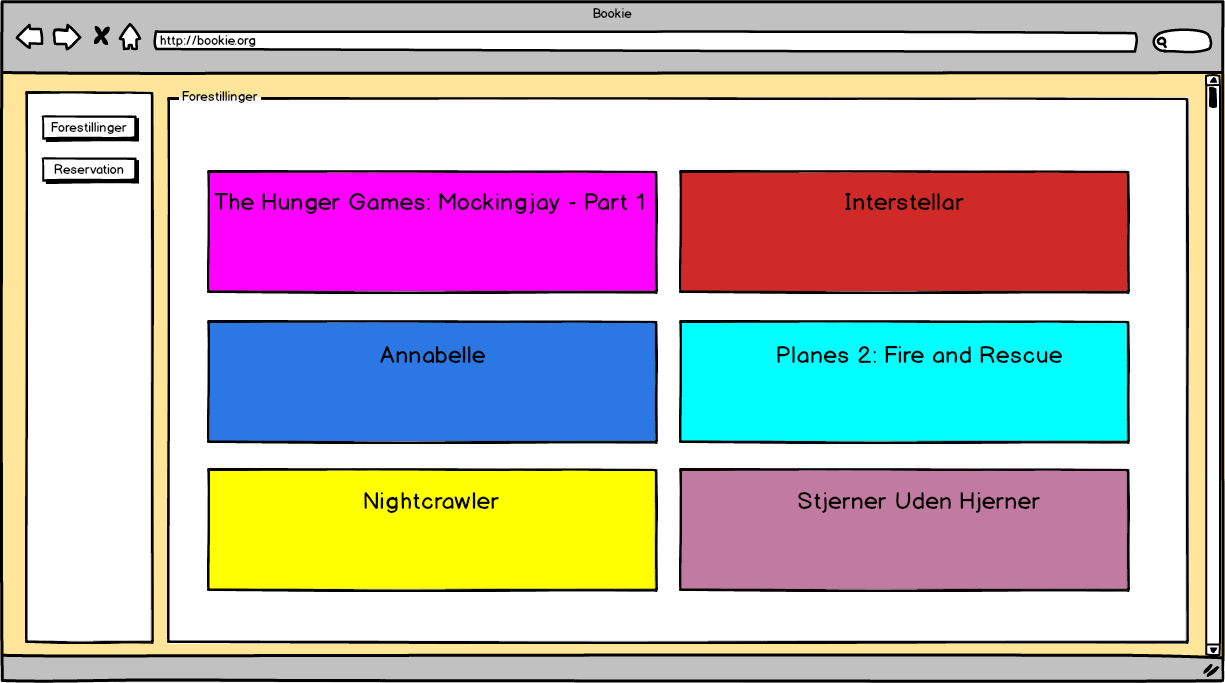
\includegraphics[width=\textwidth]{balsamiq-showtimes.png}
  \caption{Tiltænkt valg af film}
  \label{mockup:balsamiq-showtimes}
  \end{minipage}
  \hspace{0.5cm}
  \begin{minipage}[b]{0.46\linewidth}
  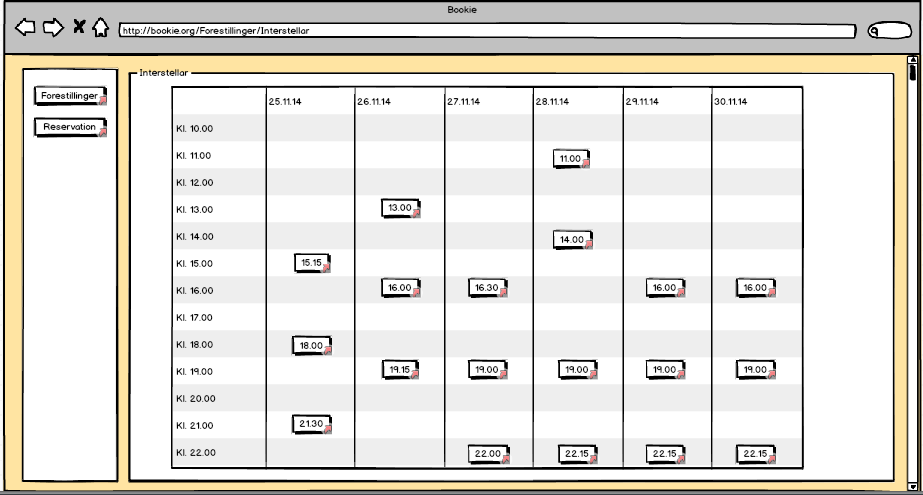
\includegraphics[width=\textwidth]{balsamiq-showtimes1.png}
  \caption{Tiltænkt valg af forestillinger}
  \label{mockup:balsamiq-showtimes1}
  \end{minipage}
\end{figure}

Ud fra vores mockup repræsenterer vi data på den måde, at der først bliver valgt en film (\ref{mockup: balsamiq-showtimes}), hvorefter man kommer ind på et vindue, hvor der er muligt at se hvilke dage og tidspunkter den valgte film bliver vist (\ref{mockup: balsamiq-showtimes1}).

\begin{figure}[h]
  \centering
  \begin{minipage}[b]{0.42\linewidth}
  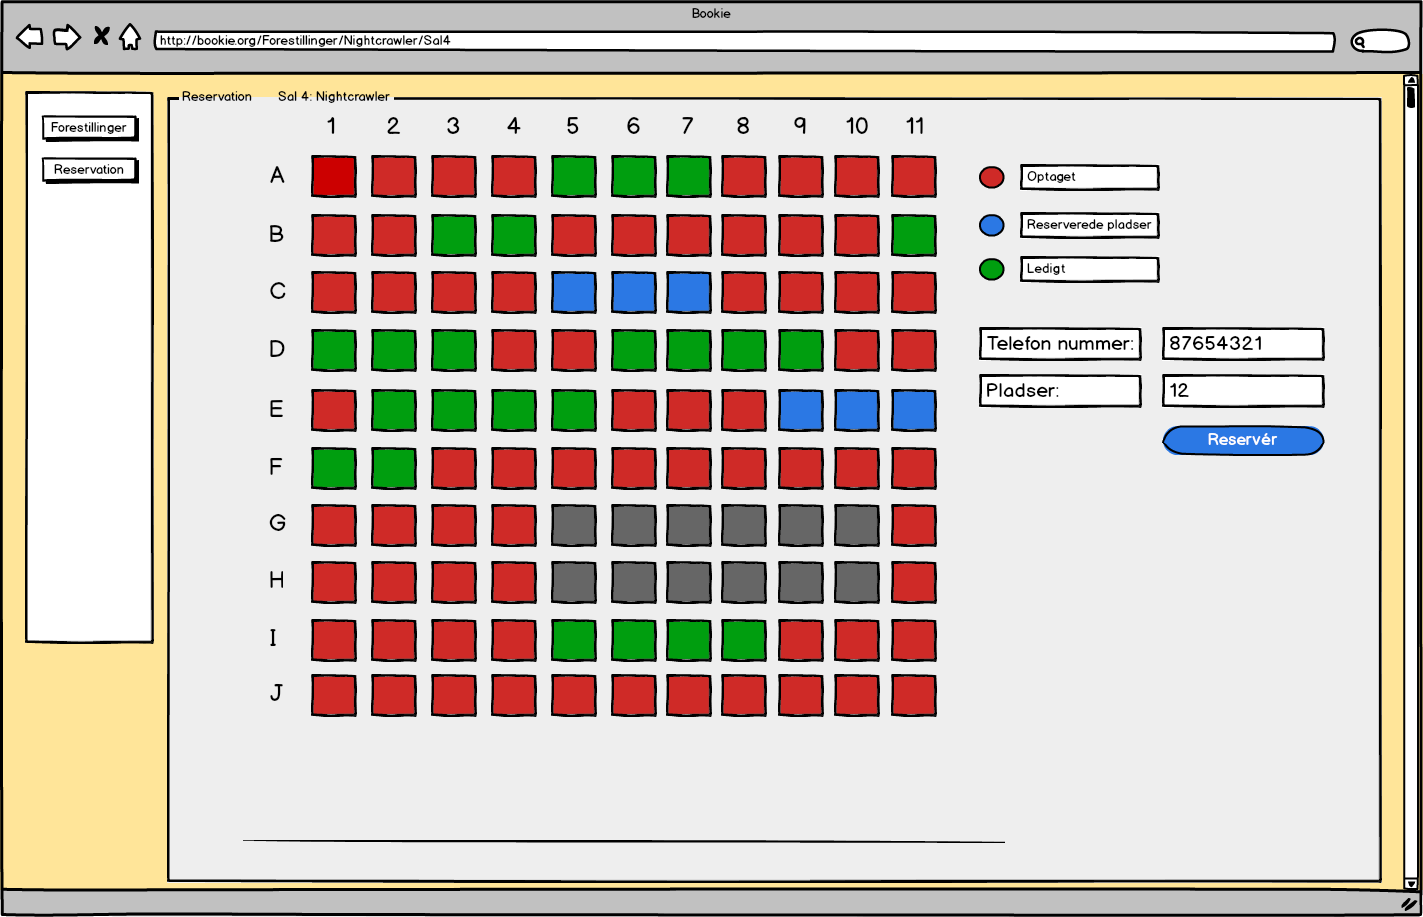
\includegraphics[width=\textwidth]{balsamiq-auditorium.png}
  \caption{Mockup - Eksempel på en sal}
  \label{mockup: balsamiq-auditorium}
  \end{minipage}
  \hspace{0.5cm}
  \begin{minipage}[b]{0.48\linewidth}
  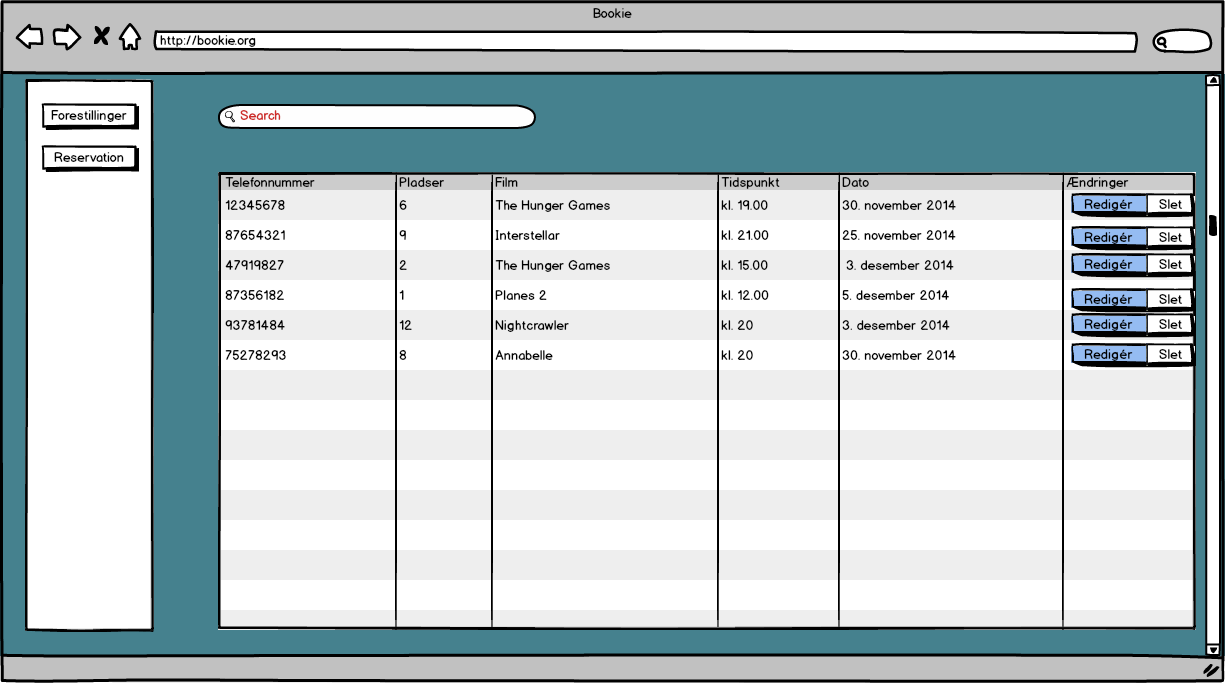
\includegraphics[width=\textwidth]{balsamiq-reservation.png}
  \caption{Mockup - Reservationer}
  \label{mockup: balsamiq-reservation}
  \end{minipage}
\end{figure}

Inde på næste vindue bliver det så muligt at reservere pladser (\ref{mockup: balsamiq-auditorium}), hvilke så ender inde på \textit{Reservationer} (\ref{mockup: balsamiq-reservation}).

I forhold til vores mockup, er der på startsiden (\ref{mockup: balsamiq-showtimes}) lavet en liste som repræsenterer filmene som data. Til hver film er der en tabel (\ref{mockup: balsamiq-showtimes1}), hvor rækkerne beskriver tidspunkter på dagen, og kolonnerne dagene i ugen. Til hver forestilling er der en sal (\ref{mockup: balsamiq-auditorium}), hvor sæderne er delt op i et gitter, og hvor hvert sæde repræsenterer en billet. Hvilket inkluderer i, at en billet er forbundet med et tidspunkt og en sal, som er forbundet til en film. Dog har \textit{Reservationer} også en liste, men denne liste indeholder billetter. Det vil sige, at billetterne også er forbundet til \textit{Reservationer}, men ikke omvendt.

Inde på \textit{Reservationer} er der også muligt at søge efter en bestemt reservation ved at skrive et telefonnummer ind på \textit{søg}-feltet. Dette felt vil så filtrere numrene i tabellen.

Idéen fungerer fint, men JavaFX har ikke samarbejdet på et optimalt plan, hvilket har fået den endelige brugergrænseflade til at blive lidt anderledes, og den har en lidt anden måde at repræsentere data på. Som det også kan ses i \textit{Brugervejledning og eksempel}, så er alle forestillinger i samme tabel, med salene til højre for tabellen. Igen er data fra reservationerne repræsenteret i et gitter. \textit{Reservationer} i Bookie minder meget om mockup'en.

\section{Systemarkitektur}
\label{chapter:systemarkitektur}

Med udgangspunkt i de tidligere beskrevne krav til reservationssystemet, ser vi god grund til at benytte os af den ofte brugte \textit{Model-view-controller} arkitektur (forkortet \textit{MVC}). Denne beskriver en streng opdeling af et systems komponenter (\cite{wiki:mvc}):

\begin{itemize}
  \item
    \textbf{Model}
  
    En Model beskriver i MVC et stykke data samt den underliggende logik for dette. Dette oversættes i reservationssystemet til de forskellige typer af data, som skal håndteres: Film, reservationer, billetter, mv.
  \item
    \textbf{View}
    
    Et View beskriver i MVC præsentationen af et systems forskellige Models. I reservationssystemet oversættes dette til de FXML-filer, som benyttes til af opbygge den visuelle del af brugergrænsefladen og dermed præsentationen af systemets data.
  \item
    \textbf{Controller}
    
    En Controller er i MVC som oftest bindeledet mellem et View og dennes bagvedliggende Model og står for at håndterede brugerinput samt at supplere Views med deres tilhørende Models. Controllere i MVC er også set brugt udelukkende som fortolker af brugerinput, og deres forhold til Models og Views er derfor ikke nødvendigvis fastdefineret (\cite{burbeck1987}).
    
    Controllere i reservationssystemet er dermed de klasser, som i systemets FXML Views måtte være refererede via \texttt{fx:controller}-attributten.
\end{itemize}
